\chapter{Cyber Threat Intelligence (CTI)}
\label{chap:Cyber Threat Intelligence}

L’Intelligence affonda le sue radici nell’ambito militare dove ha importanza strategica per prevedere e anticipare le mosse degli avversari.

Esistono numerose definizioni del termine Intelligence e tutte sono accomunate dall’importanza che hanno le informazioni. 
Conoscere le intenzioni e i mezzi del nemico è un grande vantaggio e consente di guidare in modo ottimale il processo decisionale:


\begin{itemize}
    \item\textbf{Presidenza del Consiglio dei Ministri:} Il prodotto dell’elaborazione di una o più notizie di interesse per la Sicurezza Nazionale;
    \item\textbf{NATO:} Il prodotto risultante dalla raccolta e dell’analisi delle informazioni sull’ambiente, le capacità e le intenzioni degli attori, finalizzato all’identificazione delle minacce e a supportare il processo decisionale;
    \item\textbf{FBI:} Rappresenta l’insieme di informazioni utili al processo decisionale. In qualità di membro della Comunità di Intelligence degli Stati Uniti, l’FBI raccoglie, usa e condivide tali informazioni in qualsiasi attività svolga;
\end{itemize}


La Cyber Threat Intelligence rappresenta la capacità di Intelligence sviluppata in ambito cybersecurity. Include la raccolta e l’analisi di informazioni al fine di caratterizzare possibili minacce cyber dal punto di vista tecnico, di risorse, di motivazioni e di intenti, spesso in relazione a contesti operativi specifici (Caforio, 2018).

Con la continua evoluzione delle minacce, la componente di intelligence, anche nel campo della cybersecurity, sta acquisendo un’importanza sempre più rilevante, diventando parte integrante delle strategie di difesa.

La semplificazione e l'uso improprio del termine "Cyber Threat Intelligence" possono rendere difficile per i responsabili della sicurezza valutare l'ampia gamma di opzioni disponibili per aumentare l'efficacia della sicurezza. 

\newpage

Nella migliore delle ipotesi, un'organizzazione riceve una vera e propria intelligence, che facilita decisioni proattive ed efficaci.
Nel peggiore dei casi, riceve informazioni che allo stato grezzo, non sono utilizzabili, per questo è necessario marcare la differenza tra informazioni e intelligence (Graham, 2020):


\begin{figure}[h]
\begin{center}
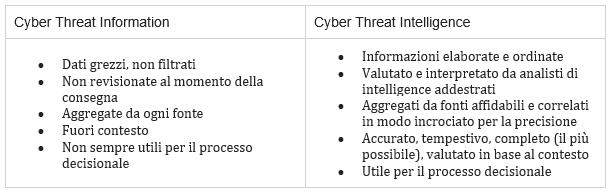
\includegraphics[width=0.95\columnwidth]{images/3_CTI_img/infoIntellDiff.png}
\end{center}
\caption{Differenze Cyber Threat Information e Cyber Threat Intelligence}
\label{fig:Differenze Cyber Threat Information e Cyber Threat Intelligence }
\end{figure}


\section{Livelli di Intelligence}
\label{sec:Livelli di Intelligence}


La cyber threat intelligence, come per l'intelligence classica, viene suddivisa in tre livelli: 

\begin{itemize}
    \item\textbf{Tattico;}
    \item\textbf{Operativo;}
    \item\textbf{Strategico;}
\end{itemize}


L'intelligence strategica informa i più alti responsabili delle decisioni, l'intelligence operativa si rivolge a coloro che prendono le decisioni quotidiane e l'intelligence tattica si concentra sulle unità che hanno bisogno di informazioni istantanee. 

\newpage

\subsection{Intelligence a livello tattico}

Questa è la forma più tecnica di intelligence, esamina cosa accade a basso livello e fornisce elementi atomici associati ad attacchi conosciuti, i famosi indicatori di compromissione (IoC).

\begin{center}
    \noindent\textbf{Esempio output intelligence tattica per APT29:}\newline\newline
    \begin{varwidth}{\textwidth}
        \begin{itemize}
          \item 628d4f33bd604203d25dbc6a5bb35b90
          \item 2aabd78ef11926d7b562fd0d91e68ad3
          \item 3d3363598f87c78826c859077606e514
          \item meek-reflect[.]appspot[.]com
          \item portal[.]sbn[.]co[.]th
          \item 202[.]28[.]231[.]44
          \item hxxps://files.counseling[.]org/eFax/incoming/150721/5442.zip
          \item googleService.exe
          \item GoogleUpdate.exe
          \item acrotray.exe
          \item PCIVEN\_80EE\&DE\_CAF
        \end{itemize}
    \end{varwidth}
\end{center}

\newpage

\subsection{Intelligence a livello operativo}

Questo livello fornisce informazioni sugli avversari, partendo dalle informazioni ricavate dall’intelligence tattica si è in grado di definire un “profilo di minaccia”, con TTP e IoC legate ad essa.

\begin{center}
    \noindent\textbf{Esempio output intelligence operativa per APT29:}\newline\newline
    \begin{varwidth}{\textwidth}
        \begin{itemize}
            \item Preferred Infection Vector: spearphishing with self-extracting RAR
            \item First Stage Malware Families: COZYCAR, SWIFTKICK, TADPOLE
            \item Second Stage Malware Families: SEADADDY, MINIDIONIS, SPIKERUSH
            \item Persistence Techniques
            \item Scheduled Tasks for most backdoors
            \item WMI by manual installation for backdoors that do not have persistence built in
            \item Legitimate file replacement of Windows Error Reporting file (wermgr.exe)
            \item Use of TOR for C2
            \item Use of Google Docs for C2
            \item Use of Google Cloud Apps for C2 forwarding (as a proxy)
            \item Use of HTTP POST requests over 443 for C2
            \item Use of backdoors configured for ports 1, 80, 443, 3389 for C2
            \item Use of PowerShell scripts
        \end{itemize}
    \end{varwidth}
\end{center}


\newpage


\subsection{Intelligence a livello strategico}

L’intelligence strategica è l’ultimo l’livello ad essere implementato, fornisce un quadro generale di come le minacce stanno mutando nel tempo. L'intelligence strategica può essere in grado di identificare tendenze storiche, motivazioni o attribuzioni su chi c'è dietro un attacco, rendendo un solido punto di partenza per decidere quali contromisure difensive saranno più efficaci.

\begin{center}
    \noindent\textbf{Esempio output intelligence strategica per APT29:}\newline\newline
    \begin{varwidth}{\textwidth}
        \begin{itemize}
            \item APT29 is a Russia-based actor that typically engages in cyber espionage with the purpose of data theft.
            \item APT29 victims include many global organizations in government, education, high-technology, finance, non-profit, pharma, and the Defense Industrial Base.
            \item APT29 is an adaptable, sophisticated group with the ability to develop custom attack tools, convoluted command-and-control infrastructure, and unlike historical behaviors of Russian state-sponsored actors, this group has the audacity to continue to operate long after they have been detected.
            \item APT29 has been historically tasked to pursue operations surrounding foreign government policy issues, especially those involving the Russia-Ukraine conflict. Furthermore, the group has targeted several Western national government agencies, defense and government contractors, and academic institutions.
        \end{itemize}
    \end{varwidth}
\end{center}

\newpage

\section{Ciclo di intelligence}
\label{sec:Ciclo di intelligence}

In generale, il processo di intelligence si compone di cinque fasi: il processo inizia con l’identificazione del fabbisogno informativo o più semplicemente con la richiesta informativa, poi vi è la raccolta delle informazioni, il trattamento delle informazioni, l’analisi, la valutazione e la produzione, la disseminazione e infine il feedback.

\begin{figure}[h]
\begin{center}
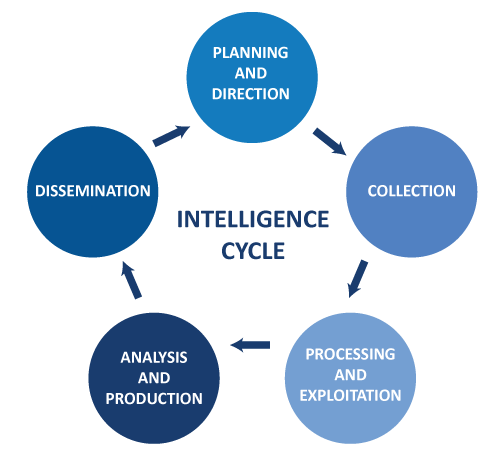
\includegraphics[width=0.80\columnwidth]{images/3_CTI_img/processoDiIntelligence.png}
\end{center}
\caption{Ciclo di intelligence}
\label{fig:Ciclo di intelligence}
\end{figure}



\subsection{Planning and direction}

Questo è probabilmente il passo più importante nel ciclo dell'intelligence, perché è il momento in cui i team definiscono lo scopo e gli obiettivi di un'operazione di intelligence, noti come requisiti di intelligence (IR).
Gli IR riflettono ciò che un team CTI non sa, ma che dovrà scoprire per soddisfare lo scopo dell'operazione.

\newpage

\subsection{Collection}

Qui viene preparato un piano di raccolta dati necessari a soddisfare le IR definite nella fase precedente.
Le principali fonti delle informazioni si suddividono in tre categorie:

\begin{itemize}
    \item\textbf{Interne:} Qualsiasi informazione raccolta dall’interno dell’organizzazione. Possono essere informazioni riportate dagli strumenti di sicurezza e dispositivi di rete (firewall, IDS, IPS) o dalle macchine e dispositivi degli utenti. Una importante parte di intelligence proviene anche da analisi forense, capace di trovare materiale non immediatamente visibile o disponibile e che può essere utile al rilevamento di altri attacchi;
    \item\textbf{Comunità:} Include qualsiasi informazione scambiata attraverso una relazione fidata con gruppi o membri che condividono lo stesso interesse. 
    \item\textbf{Esterne:} Rientrano in questa categoria le informazioni provenienti da fonti esterne all'organizzazione e non parte di un gruppo della comunità.
    A loro volta possono essere classificate in due sottocategorie:
:
        \begin{itemize}
            \item\textbf{Open Source Intelligence (OSINT):} Fonti disponibili pubblicamente, e generalmente non vi è alcun costo associato. Un esempio di un feed CTI pubblico è MalwareDomains. MalwareDomains fornisce un elenco di domini noti per essere coinvolti in attività malevole;
            \item\textbf{Close Source Intelligence (CLOSINT):} Fonti chiuse, non accessibili al pubblico. Tipicamente la consultazione avviene tramite una sottoscrizione a pagamento. Tendenzialmente la CLOSINT possiede una qualità superiore rispetto alla OSINT;
        \end{itemize} 
\end{itemize}

Ogni fonte deve essere valutata, si usa un codice che va dalla lettera “A” (affidabile) alla lettera “F” (non classificabile). Tale attività si definisce “classificazione dell’informazione”.\par
Come le fonti, anche le informazioni vanno valutate e in questo caso si usa un valore che va da “1” (confermato) a 6 (Non classificabile). Questo processo si definisce “Classificazione dei contenuti informativi” (Brando, 2018).

\newpage

\begin{figure}[h]
\begin{center}
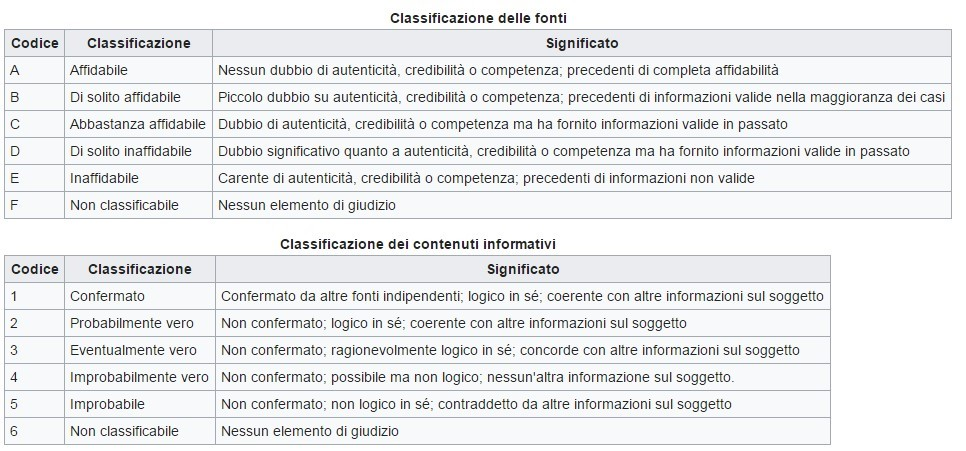
\includegraphics[width=0.95\columnwidth]{images/3_CTI_img/classificazioneInformazione.jpg}
\end{center}
\caption{Scale di classificazione delle fonti e dei contenuti informativi ricavati dal Field Manual FM 2.22-3}
\label{fig:Scale di classificazione delle fonti e dei contenuti informativi ricavati dal Field Manual FM 2.22-3}
\end{figure}

Quindi l’informazione avrà un valore dato dall’affidabilità della fonte più l’attendibilità dell’informazione. 
Ad esempio un’informazione potrebbe essere classificata come A-3, cioè la fonte si reputa “affidabile” ma non si ha certezza che la notizia sia veritiera.



\subsection{Processing and Exploitation - Analysis and Production}

Questa fase è un passaggio chiave, in quanto, trasforma i dati e le notizie raccolte in un prodotto finito utilizzabile, ed è anche il primo momento nel quale è possibile riorientare la ricerca delle informazioni.

\subsection{Dissemination}


Questo è il momento in cui l’analista comunica il risultato della sua ricerca, il quale deve esporlo in modo breve, conciso e preciso, ciò implica infatti una fase di sintesi del proprio lavoro.
La condivisione delle informazioni raccolte deve rispettare criteri di riservatezza e di formato.

\newpage

\subsubsection{Traffic Light Protocol (TLP)}

Il TLP è un protocollo utilizzato per lo scambio di informazioni in grado di garantire la diffusione delle stesse in modo controllato. 

    \begin{figure}[h]
    \begin{center}
    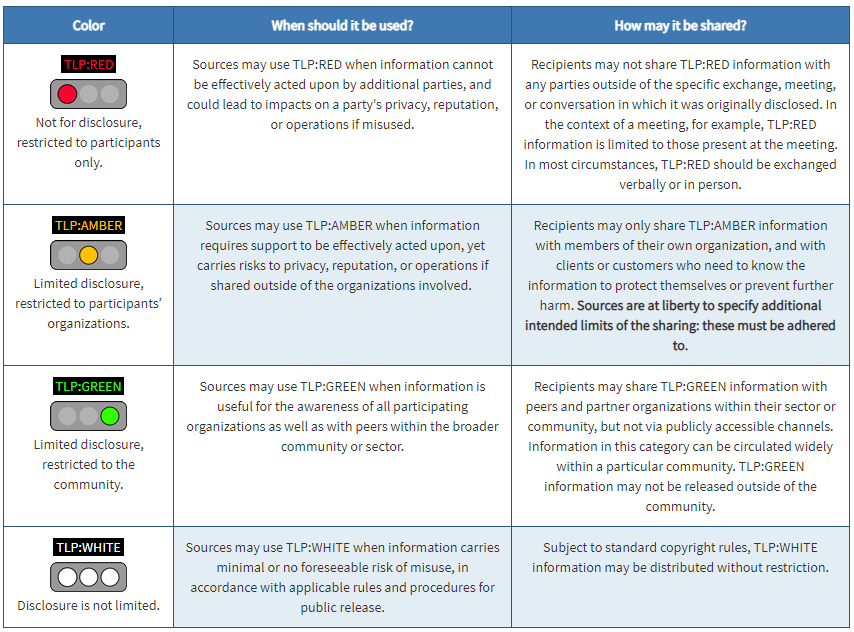
\includegraphics[width=0.95\columnwidth]{images/3_CTI_img/tlp.png}
    \end{center}
    \caption{Definizione stati del protocollo TLP}
    \label{fig:Definizione stati del protocollo TLP}
    \end{figure}
    
TLP utilizza quattro colori per indicare i limiti di condivisione, fornendo uno schema semplice e intuitivo per indicare quando e come le informazioni sensibili possono essere condivise, facilitando una collaborazione più frequente ed efficace tra entità.

\subsubsection{Standard STIX e TAXII}

Nel tempo è nata la necessità di definire uno standard strutturale per i dati di threat intelligence, al fine di agevolare la condivisione e l’utilizzo da parte delle piattaforme di sicurezza. Per risolvere questo problema sono stati sviluppati due progetti collaborativi che hanno portato alla nascita di due linguaggi open source: \textbf{STIX} e \textbf{TAXII}.

\newpage

\textbf{STIX}\newline

Structured Threat Information Expression (STIX) è un linguaggio, utilizzato per lo scambio di informazioni sulle minacce informatiche (CTI).\par
STIX consente alle organizzazioni di condividere informazioni di threat intelligence in formato standard e leggibile a livello macchina.\par
STIX nella versione 2.1, definisce 18 oggetti di tipo dato: STIX Data Objects (SDO) e 2 di tipo relazione: STIX Relationship Objects (SRO). \par
Tutti gli oggetti sono completamente opzionali e possono essere utilizzati singolarmente o insieme, a seconda dei casi d’uso.\newline

Le 18 tipologie di SDO previsti da STIX 2.1 sono:

\begin{enumerate}
    \item\textbf{Attack pattern:} Una tipologia di TTP (Tactics, Techniques and Procedures) che descrive le modalità con cui gli attori delle minacce tentano la compromissione dei target;
    \item\textbf{Campain:} Un raggruppamento di comportamenti ostili che descrive un insieme di attività malevole o attacchi che si verificano nel corso di un periodo di tempo contro una specifica categoria di target;
    \item\textbf{Course of action:} Un’azione intrapresa per prevenire o rispondere ad un attacco;
    \item\textbf{Grouping:} Afferma esplicitamente che gli oggetti STIX di riferimento hanno un contesto condiviso, a differenza di uno STIX Bundle (che non trasmette esplicitamente alcun contesto);
    \item\textbf{Identity:} Individui, organizzazioni o gruppi, così come classi di individui, organizzazioni o gruppi;
    \item\textbf{Indicator:} Contiene un pattern che può essere usato per individuare attività cyber sospette o malevole;
    \item\textbf{Infrastructure: } Rappresenta un tipo di TTP e descrive tutti i sistemi, i servizi software e le risorse fisiche o virtuali associate destinate a supportare un determinato scopo (ad esempio, server C2 utilizzati come parte di un attacco, dispositivi o server che fanno parte della difesa, server di database mirati ad un attacco, ecc.)
    \item\textbf{Intrusion set:} Un raggruppamento di comportamenti e risorse ostili con proprietà comuni che si ritiene siano orchestrate da un singolo attore;
    \item\textbf{Location:} Rappresenta una posizione geografica;
    \item\textbf{Malware:} Una tipologia di TTP, conosciuta anche come codice malevolo o software malevolo, usato per compromettere la confidenzialità, l’integrità o la disponibilità di dati o sistemi di una vittima;
    \item\textbf{Malware Analysis:} I metadati e i risultati di una particolare analisi statica o dinamica eseguita su un'istanza o una famiglia di malware;
     \item\textbf{Note:} Trasmette un testo informativo per fornire un ulteriore contesto e/o per fornire un'analisi aggiuntiva non contenuta negli oggetti STIX, negli oggetti della definizione di marcatura o negli oggetti del contenuto della lingua a cui si riferisce la nota;
    \item\textbf{Observed data:} Trasmette informazioni osservate su un sistema o una rete (es. un indirizzo IP);
    \item\textbf{Opinion:} Una valutazione della correttezza delle informazioni in un Oggetto STIX prodotto da un'altra entità;
    \item\textbf{Report:} Collezioni di threat intelligence focalizzate su uno o più argomenti, come descrizione di attori delle minacce, malware o tecniche di attacco, compresi dettagli contestuali;
    \item\textbf{Threat actor:} Individui, gruppi o organizzazioni che si ritiene possano operare con intenti malevoli;
    \item\textbf{Tool:} Software legittimo che può essere utilizzato dagli attori delle minacce per eseguire attacchi;
    \item\textbf{Vulnerability:} Un errore nel software che può essere utilizzato direttamente per ottenere l’accesso a un sistema o una rete.
\end{enumerate}

Le 2 tipologie di SRO previste da STIX 2.1 sono:

\begin{enumerate}
    \item\textbf{Relationship:} Usato per collegare due SDO e per descrivere come sono relazionati l’uno con l’altro;
    \item\textbf{Sighting:} Denota la convinzione che un elemento di Cyber threat intelligence è stato visto (es, indicatore, malware);
\end{enumerate}

   \begin{figure}[h]
    \begin{center}
    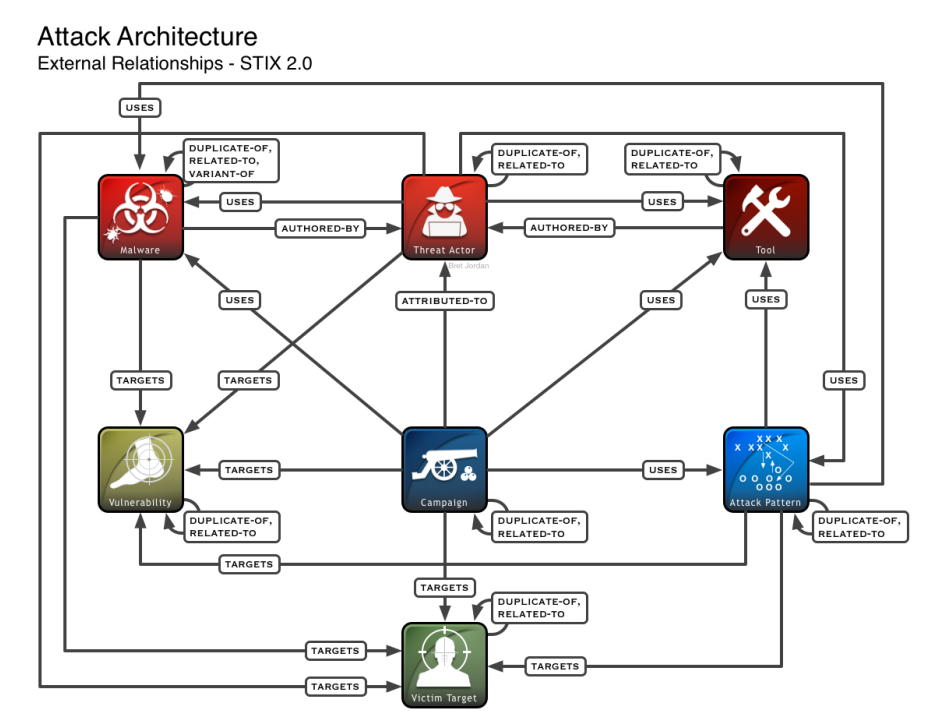
\includegraphics[width=0.90\columnwidth]{images/3_CTI_img/grafoSTIX.png}
    \end{center}
    \caption{Esempio grafo di oggetti e relazioni STIX}
    \label{fig:Esempio grafo di oggetti e relazioni STIX}
    \end{figure}

\newpage

Il modello dati di STIX può essere pensato come un grafo connesso, dove i nodi sono gli SDO e gli archi sono gli SRO. La funzione degli SRO, che rappresentano appunto gli archi del grafo, è quella di connettere gli SDO in modo che, nel tempo, gli utenti siano in grado di sviluppare e rappresentare una conoscenza più approfondita degli attori delle minacce e delle loro tecniche.\newline



\textbf{TAXII}\newline

TAXII (Trusted Automated eXchange of Indicator Information) è un progetto collaborativo che ha lo scopo di automatizzare lo scambio di informazioni di Cyber Threat Intelligence. Si tratta di un protocollo applicativo che utilizza HTTPS per lo scambio di informazioni.\par

TAXII definisce due servizi primari per supportare una varietà di modelli di condivisione comuni:



\begin{itemize}
    \item\textbf{Collection:} Una Collection è un’interfaccia ad un repository di oggetti di CTI fornite da un server TAXII che permette ad un produttore di ospitare un insieme di dati CTI che possono essere richiesti da consumatori. I client e i server TAXII scambiano informazioni attraverso un modello di tipo richiesta-risposta.
    \item\textbf{Channel:} Mantenuto da un server TAXII, un Channel permette a produttori di fornire dati a diversi consumatori e a consumatori di ricevere dati da più produttori: client TAXII scambiano informazioni con altri client TAXII in un modello pubblicatore-sottoscrittore.
\end{itemize} 

 \begin{figure}[h]
    \begin{center}
    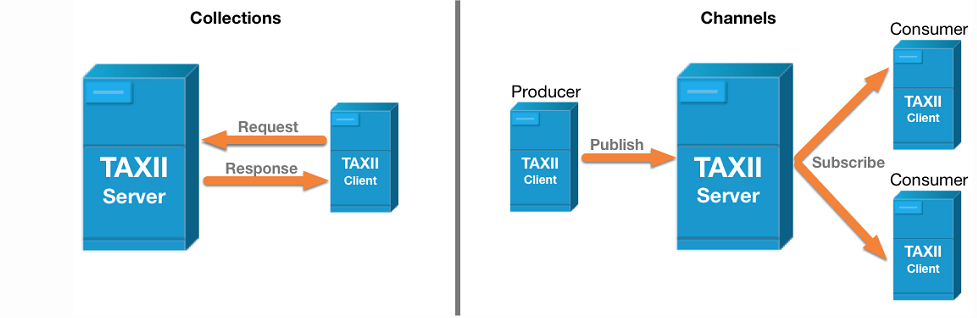
\includegraphics[width=0.90\columnwidth]{images/3_CTI_img/modelloTAXII.png}
    \end{center}
    \caption{Modelli di condivisione TAXII}
    \label{fig:Modelli di condivisione TAXII}
    \end{figure}
    
  
    
\subsection{Feedback}


Il passo finale è quando il ciclo dell'intelligence arriva a pieno regime, il che lo rende strettamente legato alla fase iniziale di pianificazione e di direzione. 
Dopo aver ricevuto il prodotto di intelligence finito, chi ha fatto la richiesta iniziale lo rivede e determina se le sue domande hanno avuto una risposta. 
Ciò guida gli obiettivi e le procedure del ciclo di intelligence successivo.

\section{Piattaforme di Threat Intelligence}
\label{sec:Piattaforme di Threat Intelligence}

Le piattaforme di Threat Intelligence, sono in grado di raccogliere dati grezzi provenienti da diverse sorgenti, sia esterne che interne, di aggregarli, arricchirli, raggrupparli, classificarli, normalizzarli, al fine di aiutare gli analisti durante il processo di intelligence, automatizzando le operazioni ripetitive.\par
L’automazione è naturalmente solo parziale, in quanto rimane fondamentale la fase di analisi, che deve essere svolta da analisti esperti con varie specializzazioni, threat analyst, incident analyst, security analyst, fraud analyst, e così via.

\newpage

Tali piattaforme possono essere integrate con strumenti di sicurezza, come: SIEM, IPS,ecc.. permettendo un continuo arricchimento della base di conoscenza di IoC  : 

 \begin{figure}[h]
    \begin{center}
    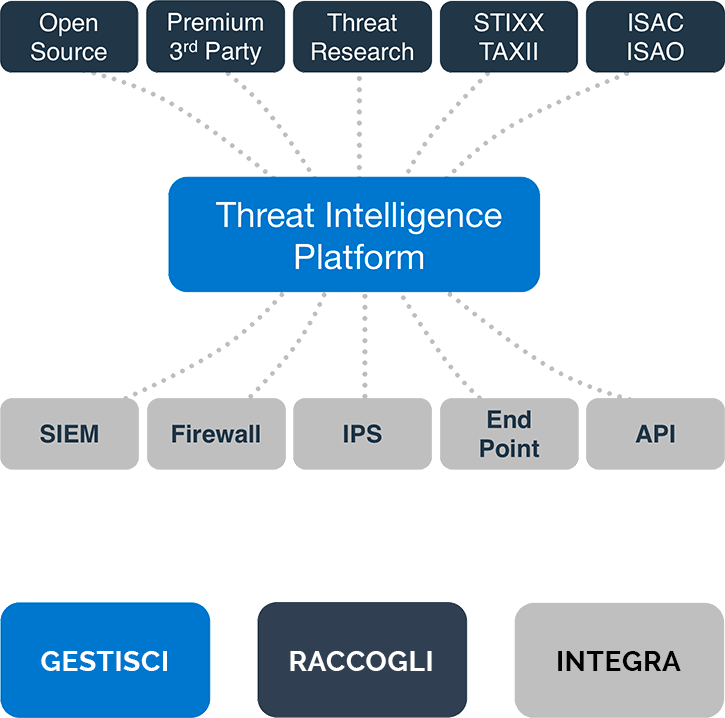
\includegraphics[width=0.80\columnwidth]{images/3_CTI_img/integrazioneTPISIEM.png}
    \end{center}
    \caption{Integrazione TIP con strumenti di sicurezza}
    \label{fig:Integrazione TIP con strumenti di sicurezza}
\end{figure}
    
    Può essere infine utile elencare le principali piattaforme di threat intelligence, limitandoci a quelle open source:
    
    \begin{itemize}
        \item\textbf{MISP:} Sviluppata dalla NATO, aiuta a tracciare ed analizzare malware. Si integra con vari IDS e firewall, con varie fonti (import ed export openIOC), vari formati (XML, CSV) ed offre API RESTful;
        \item\textbf{OpenCTI:} Originariamente sviluppato dall'ANSSI, un'agenzia francese per la sicurezza informatica in collaborazione con il CERT-EU, per migliorare le interazioni di partnership in materia di difesa della sicurezza informatica;
        \item\textbf{Alienvault Open Threat Exchange:} Open Threat Exchange è la piattaforma di Threat Intelligence da Alienvault;
        \item\textbf{IBM X-Force Exchange:} la piattaforma di Threat Intelligence fornita da IBM;
    \end{itemize}